%% Detallar aquí brevemente y con claridad, a ser posible, utilizando una figura
%% para ello, el funcionamiento del patrón MVP.
\begin{figure}[H]
	\centering
	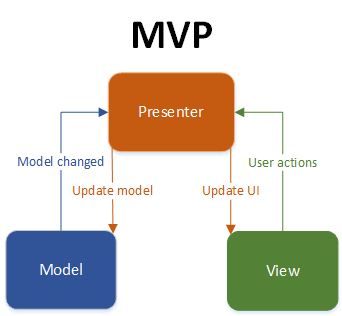
\includegraphics[width=0.6\linewidth]{mvp.png}
	\caption{Patrón Modelo-Vista-Presentador}\label{fig:mvp}
\end{figure}

Este patrón esta orientado a crear interfaces de usuario y su objetivo es separar la lógica de la aplicación de los detalles estéticos de la interfaz. Se compone de tres módulos independientes: \emph{modelo}, \emph{vista} y \emph{presentador} (ver Figura~\ref{fig:mvp}).

%% Poner Figura  


El \emph{modelo} es el encargado de gestionar los datos de la aplicación, y que de alguna forma serán mostrados al usuario. La \emph{vista} es una interfaz de usuario, normalmente gráfica, que se encarga de mostrar datos al usuario de la manera más amigable posible. Por último el presentador se sitúa entre el \emph{Modelo} y la \emph{Vista} y se encarga de conectar ambos elementos. Los eventos realizados sobre la interfaz de usuario se delegan en el presentador, que es el que decide qué cambios se deberán realizar sobre la interfaz gráfica. Para ello puede acceder a datos al modelo, o solicitar la modificación de los mismos. 

De esta forma se separa lo que es la lógica de navegación y procesamiento de eventos de los detalles de cómo se organiza exactamente una interfaz de usuario. De este modo, se aisla dicha lógica de cambios estéticos que pudiesen producrise en dicha interfaz. 

La siguiente sección mostrará como \emph{Vaadin}, un framework para el desarrollo de aplicaciones web, implementa de una manera concreta este patrón.

 


